\documentclass[11pt]{article}
\usepackage[margin=2.2cm]{geometry}
\usepackage[T1]{fontenc}
\usepackage{lmodern}
\usepackage{graphicx}
\usepackage{booktabs}
\usepackage{longtable}
\usepackage{pdflscape}
\usepackage{array}
\usepackage{verbatim}
\usepackage{xcolor}
\usepackage[hidelinks]{hyperref}
\usepackage[authoryear,round]{natbib}
% SSAbib.bst writes \citeauthoryear{full}{short}{year} (defined by the SSA class); give natbib the short form.
\providecommand{\citeauthoryear}[3]{#2(#3)}
\providecommand{\refdoi}[1]{\href{https://doi.org/#1}{#1}}
\usepackage{caption}
\captionsetup{font=small,labelfont=bf}

\graphicspath{{./figures/}}
\renewcommand{\thefigure}{S\arabic{figure}}
\renewcommand{\thetable}{S\arabic{table}}
\renewcommand{\thesection}{S\arabic{section}}
\newcommand{\file}[1]{\texttt{#1}}
\newcommand{\todo}[1]{\textcolor{red}{[#1]}}

\title{Supplemental Material for\\[4pt]
\large Recovering the 1991 Mount Pinatubo Seismic and Monitoring Record: Clocks, a Linked Catalog, and Reproducible Workflows}
\author{Glenn Thompson, John A. Power, Randall A. White and Wendy McCausland}
\date{}

\begin{document}
\maketitle

\noindent This supplement gives material that supports the main article but would crowd it: the monitoring system in more detail (Section~\ref{sec:system}), the telemetry and location settings recovered from the 1991 files (Sections~\ref{sec:telemetry} and~\ref{sec:hypo71}), the complete clock rules and further clock evidence (Section~\ref{sec:clocks}), coverage of every waveform channel and BOB product (Section~\ref{sec:coverage}), checks on the picks, locations and catalog (Section~\ref{sec:qc}), and examples from the analysis workflow (Section~\ref{sec:analysis}). Every figure and generated table is made by the notebook \file{papers/SRL/supplement/make\_supplement.ipynb} from the conversion and analysis products; all dates and times are UTC unless stated.

\section{The PVO monitoring system}\label{sec:system}

This section describes the VDAP Mobile Monitoring System as it ran at the Pinatubo Volcano Observatory (PVO) at Clark Air Base, from field sensor to analyst, using the system description of \citet{Murray_1996}, the network description of \citet{Lockhart_1996}, the manuals for the software involved \citep{Murray_1989,Murray_1990,Lee_1988,Tottingham_1989,Banfill_1999,Banfill_2003,McChesney_1999}, and the products that survive. The manuals by Banfill and McChesney describe later versions of the software and hardware; where they are cited for 1991, the corresponding features date from before 1991.

\subsection{Field stations and analog telemetry}

Each station had a short-period seismometer (Mark Products L-4 verticals; a three-component L-22D at PPO) and an amplifier and voltage-controlled oscillator (VCO) that converted the seismometer voltage into a frequency-modulated audio subcarrier. The subcarriers follow the standard USGS plan of 340~Hz spacing, 680 to 3060~Hz \citep{McChesney_1999}; each is shifted by at most about $\pm$125~Hz by the signal, so several stations can share one voice-grade radio or telephone channel. USGS analog VCOs of the period (for example the J502 and J512) used a deviation sensitivity of 115~Hz per 4.05~V and a stepped attenuator subtracted from a fixed gain \citep{McChesney_1999}; the attenuation column of the radio maps (Table~\ref{tab:radio}) records such settings. The microcontroller-based McVCO that replaced these analog VCOs dates from 1999 and was not used in 1991. \todo{Confirm the 1991 VCO model from Lockhart et al. (1996) or field notes.}

Subcarriers were combined and sent by UHF radio (about 406--418~MHz on the radio maps) to PVO. Pinatubo's ridges and canyons blocked direct line of sight from several sites, so signals were relayed: BUGZ through GRN, BURZ through PPO, and the PPO components and other channels over the Bunker Hill radio/microwave link, which was lost on 11 June (Figure~\ref{fig:telemetry}, Table~\ref{tab:radio}). Analog FM telemetry has no bit depth; its dynamic range, limited by the subcarrier deviation and the noise of the radio path, is commonly quoted as about 40--50~dB, below that of the 12-bit digitizers at PVO. \todo{Cite a source for the telemetry dynamic range.}

\subsection{Demodulation and digitization at PVO}

At PVO the radio receivers fed a rack of discriminators, one per subcarrier, which demodulated each channel back to an analog voltage proportional to the seismometer signal (Figure~2 of the main article). The discriminator outputs drove the helicorders, which kept their own clock, and were split to the analog-to-digital converters (ADCs) of the acquisition computers, each with its own clock:
\begin{itemize}
\item \textbf{WILLIE} (IBM-AT) ran MDETECT \citep{Lee_1988,Tottingham_1989}, which digitized all seismic channels with a 12-bit ADC at a nominal 100 samples/s (3125/31~Hz in the surviving files), detected events and wrote triggered, multiplexed SUDS (DMX) files \citep{Ward_1989}. MDETECT kept time by counting samples from the PC clock read at start-up. One channel carried an IRIG time code from a free-running generator; in later SUDS processing the Irig program decodes an IRIG-E channel to correct the start time and sampling rate \citep{Banfill_1999}, but with a free-running generator this gives no absolute time. WILLIE also ran SSAM, which wrote one-minute spectral amplitudes in 16 bands for selected channels. \todo{ADC board model and channel count; SSAM program reference.}
\item \textbf{The Tandy Model 100} ran RSAM \citep{Murray_1989}. Its acquisition board buffers up to eight discriminator outputs per board (up to three boards per Tandy), high-passes them at 0.1~Hz, rectifies them and digitizes them with an 8-bit ADC at about 50 samples/s per input. The program averages the rectified amplitude each minute and sends 10-minute averages, in ``RSAM units'', to a host computer over RS-232. It also counts ``RSAM events'': a two-second amplitude that exceeds the one before last by a set ratio (default 2) and a threshold. The published program counts events on three channels only; the surviving EVNT files likewise have exactly three channels on 197 of their 206 days (Figure~\ref{fig:bobrsam}).
\item \textbf{SLEEPY} (IBM-XT) logged tilt (tilt components, battery voltage and temperature at PPO and UBO) every 10 minutes.
\item \textbf{RICKY} (IBM-XT) logged the acoustic flow monitors installed on lahar channels from mid-1991, and we infer rainfall as well (main article).
\end{itemize}
The acquisition PCs sent their products through a buffered serial printsharer to the aggregation PC (PORKY), and WILLIE's event files went over a 2~Mb/s peer-to-peer LAN to the analysis PCs; a 9600-baud modem on ANDY gave remote access from the Cascades and Alaska volcano observatories \citep{Murray_1996}. No step of this chain synchronized the clocks, which is why each product needs its own clock rule.

\subsection{From trigger to location}

MDETECT, like XDETECT \citep{Tottingham_1989}, triggered on the ratio of short- to long-term average amplitudes on each channel and declared a network event when enough channels triggered together, saving a pre-event buffer and the following record as one DMX file. \todo{Check the MDETECT trigger parameters against Lee et al. (1988).} Analysts then reviewed the triggered files: they demultiplexed them, displayed them and picked P and S arrivals (and coda durations) in SUDSPICK \citep{Banfill_1999}, and located the events with HYPO71 \citep{Lee_1975} using the control file in Section~\ref{sec:hypo71}. The picks survive as phase (PHA) files and the locations as the two HYPO71 summaries described in the main article. Event classes (for example long-period and hybrid events) were noted by hand in a written logbook and are not part of the digital record. \todo{Logbook: does it survive, and where?}

\subsection{BOB: archiving and display}

The aggregation PC stored the low-rate products (RSAM, EVNT, SSAM, tilt, lahar, rain and hand-entered values such as COSPEC SO$_2$ fluxes and daily event counts) in the BOB data system \citep{Murray_1990}. BOB data files are direct-access binary files holding one year of one measurement at a fixed rate (for example 144 points per day for 10-minute data), with $-$998 marking a missing value; aperiodic data such as COSPEC are kept in sequential files with a time for each value. These are the ``annual binary'' files of Table~1 in the main article, and $-$998 is the missing-value code found throughout the recovered BOB products.

BOB loads data into eight columns (A--H), where they can be averaged, offset, scaled and corrected without changing the stored files, and plots up to eight panels against a common time axis, for example \texttt{PLOT 3 A B C} for three stacked panels, with \texttt{+} overlaying two columns in one panel \citep{Murray_1990}. Command sequences are saved as macros, which can be nested and called from menus, so that a non-specialist could display, for instance, the last 24 hours of 10-minute RSAM, or rain, mudflow, event rates, RSAM and COSPEC as separate panels over the same days. The \texttt{LAST} command takes its end time from the computer's clock: a BOB plot is labelled in whatever time the aggregation PC was set to, independently of the clocks that stamped the data.

\section{Telemetry}\label{sec:telemetry}

Figure~\ref{fig:telemetry} shows the documented pre-eruption telemetry routes; Table~\ref{tab:radio} lists the three dated radio-frequency maps recovered with the BOB archive (step 68). Each discriminator slot at PVO received one channel; the VCO centre frequency identifies its audio subcarrier and the radio frequency its UHF link. Channels sharing a radio frequency were multiplexed on one link, for example the PPO components on the ``Volcano 1 phone'' path and BUGZ relayed through GRNZ.

\begin{figure}[htbp]
\centering
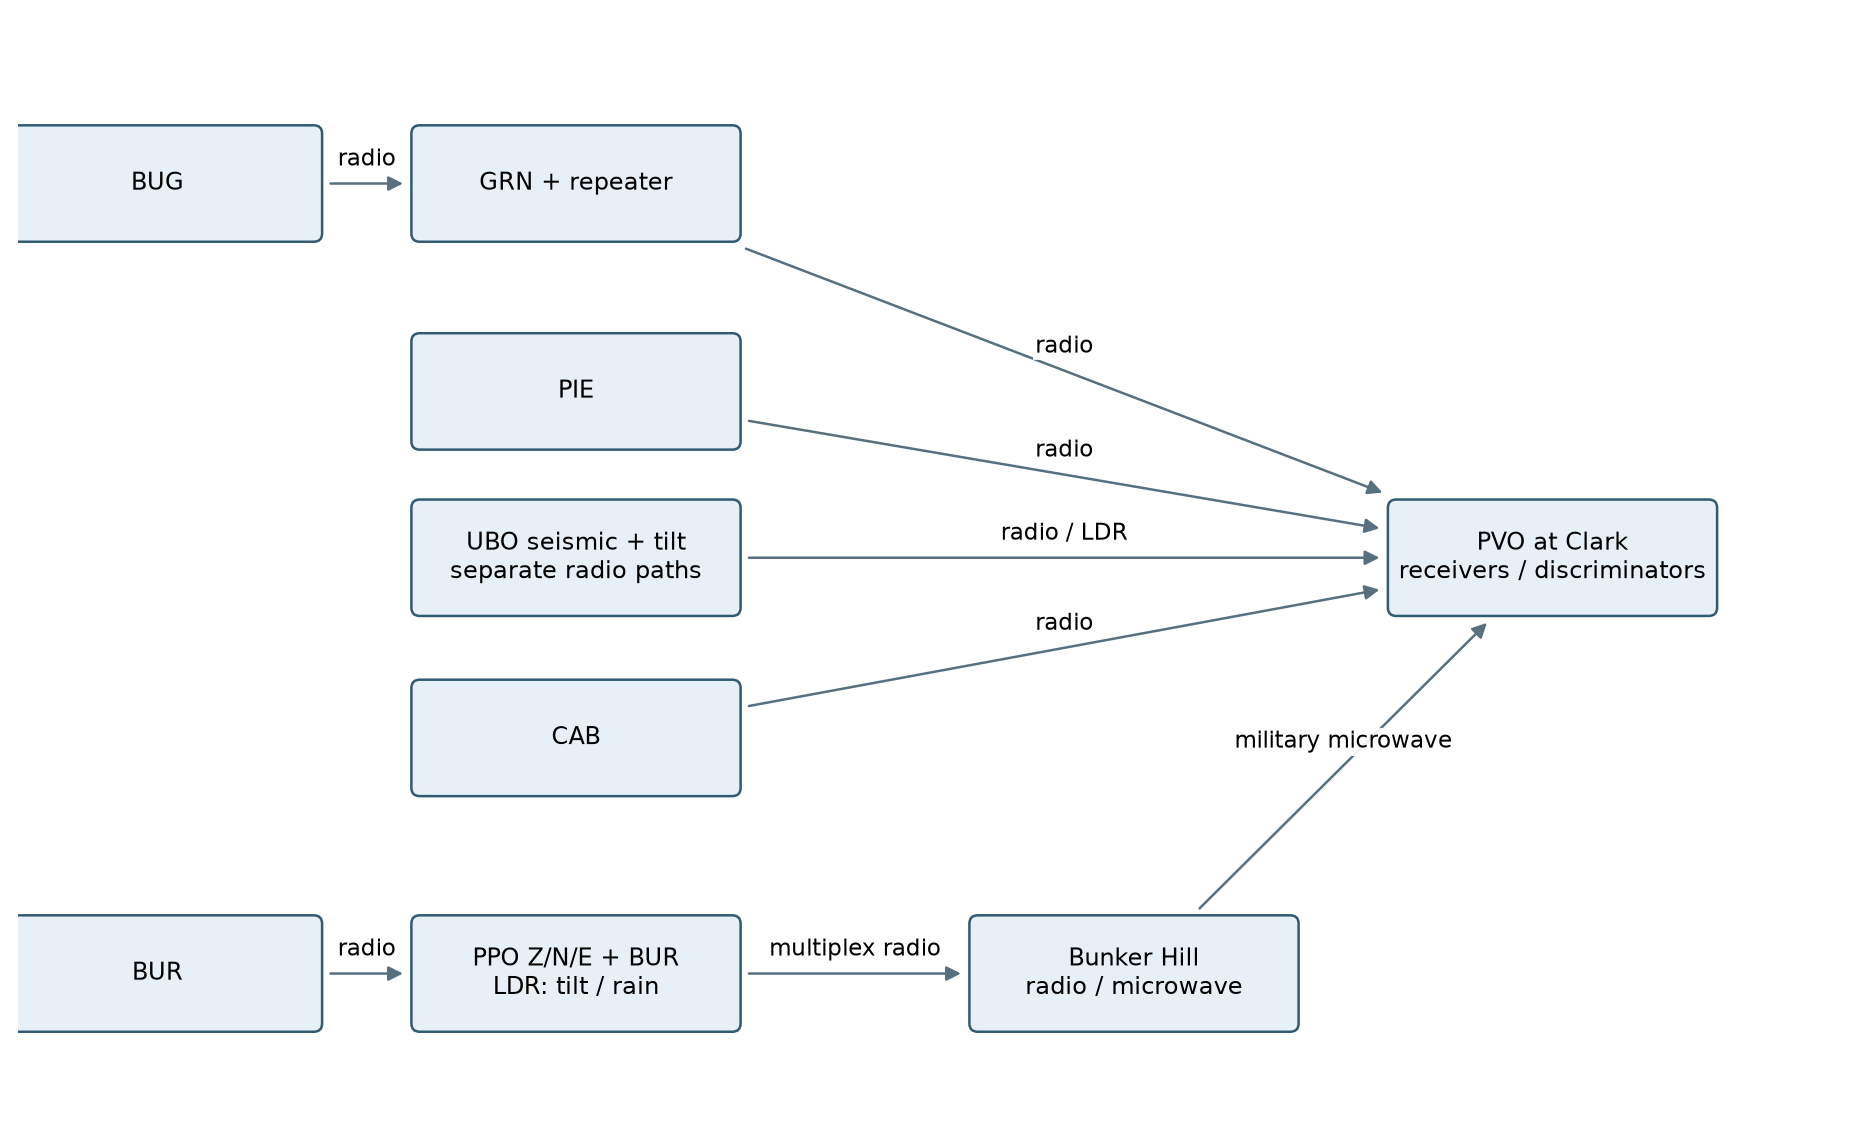
\includegraphics[width=\textwidth]{figS01_telemetry}
\caption{Documented pre-eruption telemetry, schematic rather than geographic \citep[after][]{Lockhart_1996,Murray_1996}. The Bunker Hill link was lost on 11 June; an attempt to use Crow's Nest on 14 June failed and is not shown as a route. The rebuilt July--August routes are not reconstructed, and no links are inferred from station coordinates.}
\label{fig:telemetry}
\end{figure}

{\footnotesize
\setlength{\tabcolsep}{3pt}
\begin{longtable}{lllllll}
\caption{Radio-frequency maps as written: discriminator slot, channel, site, attenuation (dB), VCO centre frequency (Hz), radio frequency (MHz) or link, and relay. A ditto mark (") repeats the line above. The \file{SEIS\_MAP.CUR} copy of the 8 July map is identical and is not repeated.}\label{tab:radio}\\
\toprule
Slot & Channel & Site & Atten. & VCO & Radio & Relay\\
\midrule\endfirsthead
\toprule
Slot & Channel & Site & Atten. & VCO & Radio & Relay\\
\midrule\endhead
\bottomrule\endfoot
\multicolumn{7}{l}{\textbf{14 May 1991}}\\
01 & GRNZ & Negron &  & 1700 & 406.28125 & \\
02 & UBOZ & Pinatubo &  & 1020 & 409.86875 & \\
03 & PIEZ & Pinatubo East &  & 1360 & 417.675 & \\
04 & PPOE & Patal Pinto (east Comp.) &  & 2720 & 412.075 & VOLCANO 1 PHONE\\
05 & PPOZ & Patal Pinto (vertical Comp.) &  & 1360 & " & \\
06 & BURZ & Burgos &  & 2380 & 408.50625 & PPO\\
07 & PPON & Patal Pinto (north Comp.) &  & 1020 & 412.075 & VOLCANO 1 PHONE\\
08 & CABZ & Clark Air Base &  & 3060 & 416.80625 & \\
09 & BUGZ & Buag Sitio &  & 680 & 408.90125 & GRNZ\\
\multicolumn{7}{l}{\textbf{27 June 1991}}\\
01 & FNGZ & 6 Km East Of Negron &  & 2380 & 406.281 & \\
02 & QADZ & Mt. Cuadrado &  & 2040 & 408.981 & \\
03 & DONZ & Camp O'donnell &  & 2720 & VOLCANO 1 PHONE & \\
04 & PI2Z & Pinatubo East \#2 Normal Gain &  & 1700 & 411.825 & \\
05 & PI2L & " Low Gain &  & 2720 & " & \\
06 & ---- &  &  &  &  & \\
07 & ---- &  &  &  &  & \\
08 & CABZ & Clark Air Base &  & 3060 & 416.80625 & \\
09 & ---- &  &  &  &  & \\
\multicolumn{7}{l}{\textbf{8 July 1991}}\\
01 & FNGZ & 6 Km East Of Negron & 36 & 2380 & 406.281 & \\
02 & QADZ & Mt. Cuadrado & 36 & 2040 & 408.981 & \\
03 & DONZ & Camp O'donnell & 36 & 2720 & VOLCANO 1 PHONE & \\
04 & PI2Z & Pinatubo East \#2 Normal Gain & 36 & 1700 & 411.825 & \\
05 & PI2L & " Low Gain & ? & 2720 & " & \\
06 & CRWZ & Crow's Nest & 36 & 1020 & 416.806 & PI2\\
07 & BUGZ &  & 36 & 2040 & 416.79375 & QAD\\
08 & CABZ & Clark Air Base Vertical & 24 & 3060 & 416.806 & \\
09 & CABE & " East-west & ? & 1700 & " & \\
10 & CABN & " North-south & ? & 2040 & " & \\
\end{longtable}
}


\section{HYPO71 settings}\label{sec:hypo71}

A set of HYPO71 \citep{Lee_1975} control cards was recovered from the June 1991 monthly phase file, where it appears in the gap in picks between 10 and 27 June (saved as \file{hypo71\_settings\_199106.txt} in \file{10\_conversion}). It gives the reset test variables, sixteen station cards and a five-layer P-velocity model with $V_P/V_S = 1.78$ (Table~\ref{tab:model}). Whether every 1991 location used this model is not known; the two surviving summaries do not record their control files.

\begin{table}[htbp]
\centering
\caption{HYPO71 P-velocity model from the June 1991 control cards.}\label{tab:model}
\begin{tabular}{rrr}
\toprule
$V_P$ (km/s) & Top (km) & Bottom (km)\\
\midrule
3.30 & 0.0 & 1.0\\
5.00 & 1.0 & 4.0\\
5.70 & 4.0 & 15.0\\
6.70 & 15.0 & 25.0\\
8.00 & 25.0 & $\infty$\\
\bottomrule
\end{tabular}

\end{table}

\noindent The control file as recovered:
{\scriptsize\verbatiminput{tables/hypo71_settings_199106.txt}}

\section{Clock rules and further evidence}\label{sec:clocks}

Table~\ref{tab:clockrules} reproduces \file{clock\_regimes.csv}, the rules applied by every conversion step. The main article summarizes the evidence; Figures~\ref{fig:evnt}--\ref{fig:anchors2} add two independent checks.

\begin{landscape}
{\scriptsize
\setlength{\tabcolsep}{3pt}
\begin{longtable}{>{\raggedright}p{2.7cm}>{\raggedright}p{2.6cm}c>{\raggedright}p{1.6cm}>{\raggedright}p{1.6cm}>{\raggedright}p{2.9cm}rrrl>{\raggedright\arraybackslash}p{5.5cm}}
\caption{Clock rules (\file{10\_conversion/clock\_regimes.csv}). Start and end are on the stream's own raw clock, half-open; offsets in hours (UTC = raw + offset), uncertainties in seconds. Sequence and marker apply only around the 26 May reset.}\label{tab:clockrules}\\
\toprule
Stream & Rule & Clock & Start & End & Sequence & Marker & Offset & Unc. & Conf. & Evidence\\
\midrule\endfirsthead
\toprule
Stream & Rule & Clock & Start & End & Sequence & Marker & Offset & Unc. & Conf. & Evidence\\
\midrule\endhead
\bottomrule\endfoot
waveform & H\_\allowbreak{}PHT & H &  & 1991-05-26 16:45:00 & 91052617 & 0 & -15 & 60 & high & Old MDETECT (DMX localtime 0); PC clock on PHT; hypocenters = H - 7 h; RSAM labels (PHT) = H - 7 h 10-26 May; last file 91052617 (H 15:41:33)\\
waveform & H\_\allowbreak{}UTC\_\allowbreak{}PDT & H & 1991-05-26 07:40:00 & 1991-10-27 09:00:00 & 9105261G & -25200 & -7 & 25 & high & New MDETECT (DMX localtime -25200) from 9105261G (H 08:40:26 = PINAALL line 218 + 7 h); PC clock on GMT; filename date = date(H - 7 h); RSAM labels (PHT) = H + 1 h\\
waveform & H\_\allowbreak{}UTC\_\allowbreak{}PST & H & 1991-10-27 09:00:00 &  & 9105261G & -25200 & -8 & 25 & high & US DST ended 27 Oct 1991 02:00 PDT; filename date = date(H - 8 h) from 28 Oct; EVNT lag steps -7 h to -8 h\\
pick\_individual; pick\_monthly; hypo\_brun & H\_\allowbreak{}PHT & H &  & 1991-05-26 07:40:00 &  &  & -15 & 60 & high & Picks on the header clock before the reset\\
pick\_individual & H\_\allowbreak{}PHT\_\allowbreak{}seq & H & 1991-05-26 07:40:00 & 1991-05-26 16:45:00 & 91052617 &  & -15 & 60 & high & Last file before the reset is 91052617\\
pick\_individual & H\_\allowbreak{}UTC\_\allowbreak{}seq & H & 1991-05-26 07:40:00 & 1991-05-26 16:45:00 & 9105261G &  & -7 & 25 & high & First file after the reset is 9105261G\\
pick\_individual & H\_\allowbreak{}UTC\_\allowbreak{}PDT & H & 1991-05-26 16:45:00 & 1991-10-27 09:00:00 &  &  & -7 & 25 & high & Single-event PHA files (3-16 June): 100\% inside waveform windows on H\\
pick\_monthly; hypo\_brun & H\_\allowbreak{}PHT\_\allowbreak{}seq & H & 1991-05-26 07:40:00 & 1991-05-26 16:45:00 & pinmay91.pha:005541 &  & -15 & 60 & high & pinmay91.pha has no pre-reset picks in the repeated window\\
pick\_monthly; hypo\_brun & H\_\allowbreak{}UTC\_\allowbreak{}seq & H & 1991-05-26 07:40:00 & 1991-05-26 16:45:00 & pinmay91.pha:005542 &  & -7 & 25 & high & pinmay91.pha line 5542 onward matches post-reset files 9105261H...\\
pick\_monthly; hypo\_brun & H\_\allowbreak{}UTC\_\allowbreak{}PDT\_\allowbreak{}until\_\allowbreak{}switch & H & 1991-05-26 16:45:00 & 1991-06-10 12:00:00 &  &  & -7 & 25 & high & Monthly picks on H up to 10 June 00:06 (100\% inside waveform windows)\\
pick\_monthly; hypo\_brun & W\_\allowbreak{}UTC & W & 1991-06-20 00:00:00 &  &  &  & 0 & 25 & medium & From 27 June monthly picks are on W (88-100\% inside waveforms at +7 h); new HYPO71 control cards in pinjun91.pha lines \textasciitilde{}5632-5666; no picks between 10 and 27 June\\
hypo\_pinaall; hypo\_allsum; hypo\_gold; hypo\_pepi & W\_\allowbreak{}PHT & W &  & 1991-05-26 00:40:00 &  &  & -8 & 60 & high & Hypocenters = H - 7 h = W; W was PHT before the reset\\
hypo\_pinaall; hypo\_allsum; hypo\_gold; hypo\_pepi & W\_\allowbreak{}PHT\_\allowbreak{}seq & W & 1991-05-26 00:40:00 & 1991-05-26 09:45:00 & 000217 &  & -8 & 60 & high & PINAALL.DAT line 217 (08:31:25) is the last pre-reset record\\
hypo\_pinaall; hypo\_allsum; hypo\_gold; hypo\_pepi & W\_\allowbreak{}UTC\_\allowbreak{}seq & W & 1991-05-26 00:40:00 & 1991-05-26 09:45:00 & 000218 &  & 0 & 25 & high & PINAALL.DAT line 218 (01:40:38) is the first post-reset record (= 9105261G - 7 h)\\
hypo\_pinaall; hypo\_allsum; hypo\_gold; hypo\_pepi & W\_\allowbreak{}UTC & W & 1991-05-26 09:45:00 &  &  &  & 0 & 25 & high & Wall clock on GMT after the reset\\
tandy\_rsam & R\_\allowbreak{}ahead & R &  & 1991-05-09 06:00:00 &  &  & -15 & 10800 & low & 2-9 May EVNT/RSAM cross-correlation: R = H (unexplained); switch between 9 May 00-06 and 06-12 R\\
tandy\_rsam & R\_\allowbreak{}PHT & R & 1991-05-09 06:00:00 & 1991-09-13 09:00:00 &  &  & -8 & 300 & high & R = H - 7 h (10-26 May) and H + 1 h (26 May-13 Sep) = PHT; eruption onsets; switch times +-3 h\\
tandy\_rsam & R\_\allowbreak{}GMT & R & 1991-09-13 09:00:00 & 1991-11-10 00:00:00 &  &  & 0 & 300 & medium & R = H - 7 h from 13 Sep (06-12 R) and H - 8 h after 28 Oct = UTC; RSAM = summed SSAM within 0-3 min on every day\\
tandy\_rsam & R\_\allowbreak{}PHT\_\allowbreak{}10Nov & R & 1991-11-10 00:00:00 & 1991-11-11 00:00:00 &  &  & -8 & 300 & high & RSAM PC (Tandy) on local time: the RSAM block of 10 Nov (labels 01:20-22:20 R) matches summed SSAM 8 h earlier on all 5 stations (r 0.92-0.94; 0 h: r < 0) and EVNT matches waveform triggers at -8 h (r 0.59); SSAM and RSAM both resume about 9 Nov 17:10 UTC\\
tandy\_rsam & R\_\allowbreak{}GMT\_\allowbreak{}after\_\allowbreak{}10Nov & R & 1991-11-11 00:00:00 &  &  &  & 0 & 300 & medium & RSAM = summed SSAM within 0-3 min from 14 Nov; weak EVNT correlation after \textasciitilde{}7 Nov\\
ssam & W\_\allowbreak{}PHT & W &  & 1991-05-26 09:45:00 &  &  & -8 & 60 & medium & MDETECT/SSAM PC on PHT before the reset; no SSAM data before 1 June, row kept for completeness\\
ssam & W\_\allowbreak{}UTC & W & 1991-05-26 09:45:00 &  &  &  & 0 & 60 & high & SSAM and SSAM DATA labels = RSAM label - 8 h until 13 Sep and = RSAM label after (station-matched cross-correlation, r = 0.72-0.99), i.e. GMT throughout like the MDETECT PC after the reset; 1-min labels\\
sleepy\_tilt & T\_\allowbreak{}PHT & T &  &  &  &  & -8 & 3600 & medium & SLEEPY (tilt acquisition PC). Labels are PHT: PBAT battery charging starts at the 07:00 label and peaks at 11-14 on every day (solar day in PHT, not GMT); TIME.TXT and BOB\_UBO\_.TXT: files phased by 48 samples (8 h) from GMT to local on 18 Nov 91 (Murray); values only 1-13 June\\
ricky\_lahar & L\_\allowbreak{}PHT & L &  & 1991-09-13 09:00:00 &  &  & -8 & 600 & high & Mudflow vs RSAM (UTC): best lag -8 h for USAC, GUMA, MARL (r 0.4-0.7, Jul-12 Sep); rain increments match RSAM at -7/-8 h and mudflow at 0 h; hours 00-07 carry the correct date; switch found independently at 12-15 Sep\\
ricky\_lahar & L\_\allowbreak{}GMT & L & 1991-09-13 09:00:00 & 1991-11-15 00:00:00 &  &  & 0 & 600 & medium & Mudflow vs RSAM best lag 0 from 15 Sep (r 0.4-0.7 to October) although the files still say converted from GMT to local; rain vs RSAM and mudflow lag 0; 1-14 Nov untested (no lahar signal)\\
cab\_hourly\_counts & C\_\allowbreak{}PHT & C &  & 1991-09-13 09:00:00 &  &  & -8 & 1800 & medium & Hourly CAB counts entered by hand (header says TIME IN GMT): vs EVNT (UTC) best lag -8 h in most weeks from 23 Jun to 12 Sep (r up to 0.49; June-July weak); hh:30 labels are hour centres\\
cab\_hourly\_counts & C\_\allowbreak{}GMT & C & 1991-09-13 09:00:00 &  &  &  & 0 & 1800 & medium & vs EVNT best lag 0 from 15 Sep (r 0.64, 0.45) and late October (r 0.37); switch between the weeks of 8 and 15 Sep\\
\end{longtable}
}
\end{landscape}


\begin{figure}[htbp]
\centering
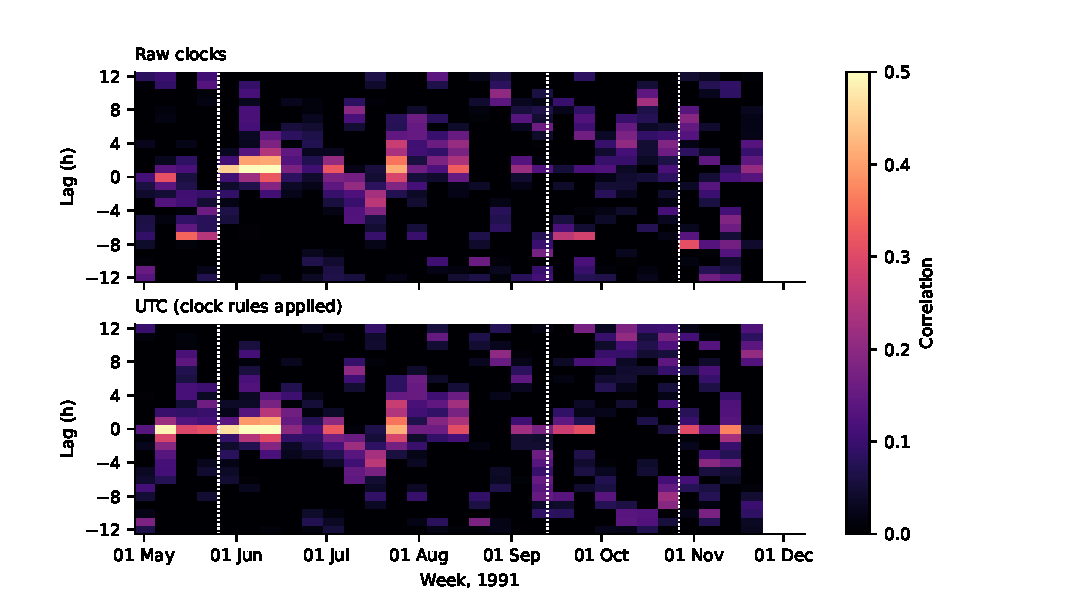
\includegraphics[width=\textwidth]{figS02_evnt_trigger_lag}
\caption{Correlation between hourly EVNT trigger counts (Tandy RSAM PC) and hourly counts of triggered waveform records (WILLIE), week by week, at lags of $\pm$12~h. Square-root counts with a 24-h running mean removed. Top: raw clocks. The ridge lies at $-$7~h before the 26 May reset (both PCs on Philippine time, but the DMX header clock is the wall clock + 7~h), at +1~h until 13 September (RSAM PC on Philippine time, UTC+8; header clock UTC+7), at $-$7~h once the RSAM PC moved to GMT, and at $-$8~h after daylight time ended on 27 October. Bottom: after the clock rules, 0~h throughout. Dotted lines: 26 May, 13 September, 27 October.}
\label{fig:evnt}
\end{figure}

\begin{figure}[htbp]
\centering
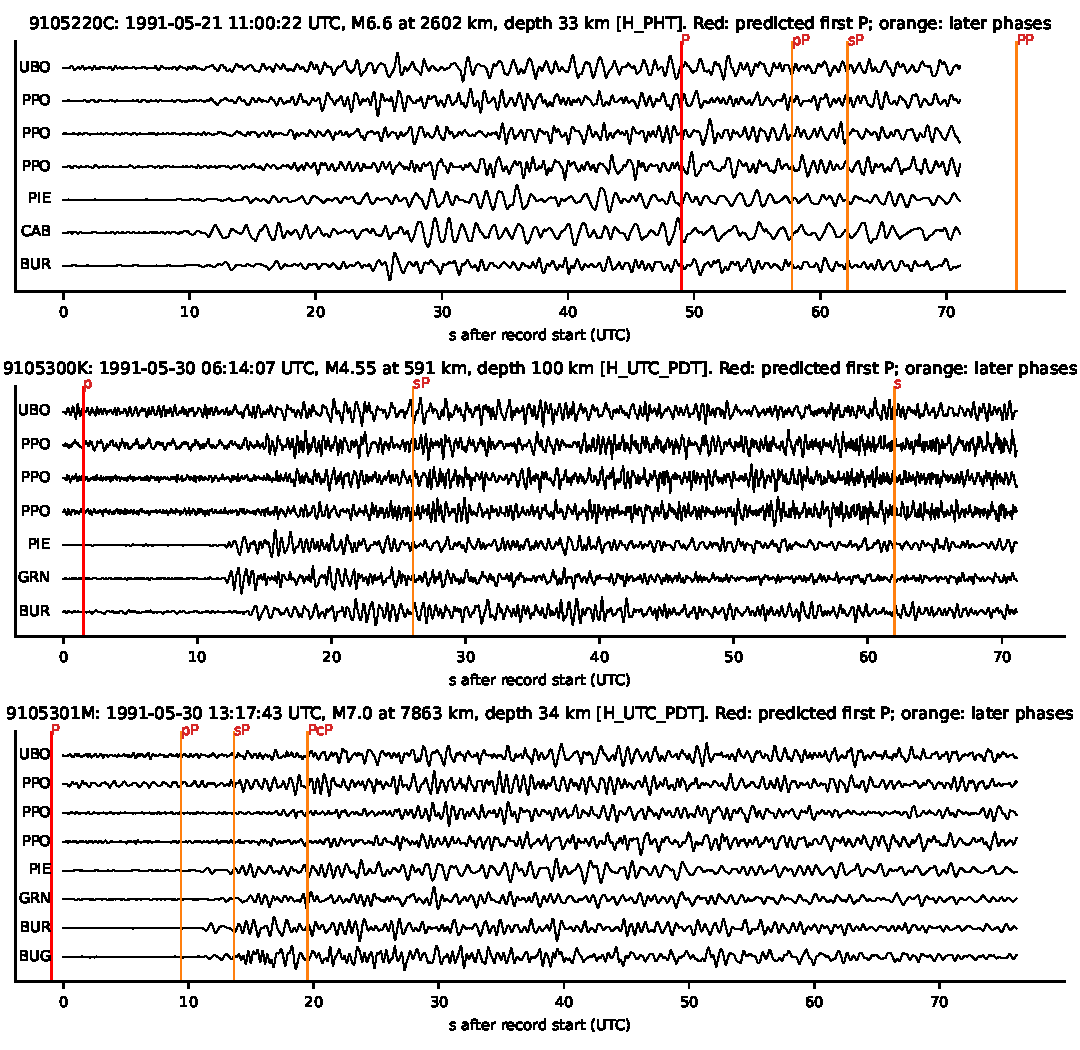
\includegraphics[width=\textwidth]{figS03_anchors_may}
\caption{Clock anchors before and after the reset, May 1991 (step 72): records 9105220C, 9105300K and 9105301M with the predicted P arrival (iasp91) from the ISC/USGS origin. See Table~3 of the main article for the measured offsets.}
\label{fig:anchors1}
\end{figure}

\begin{figure}[htbp]
\centering
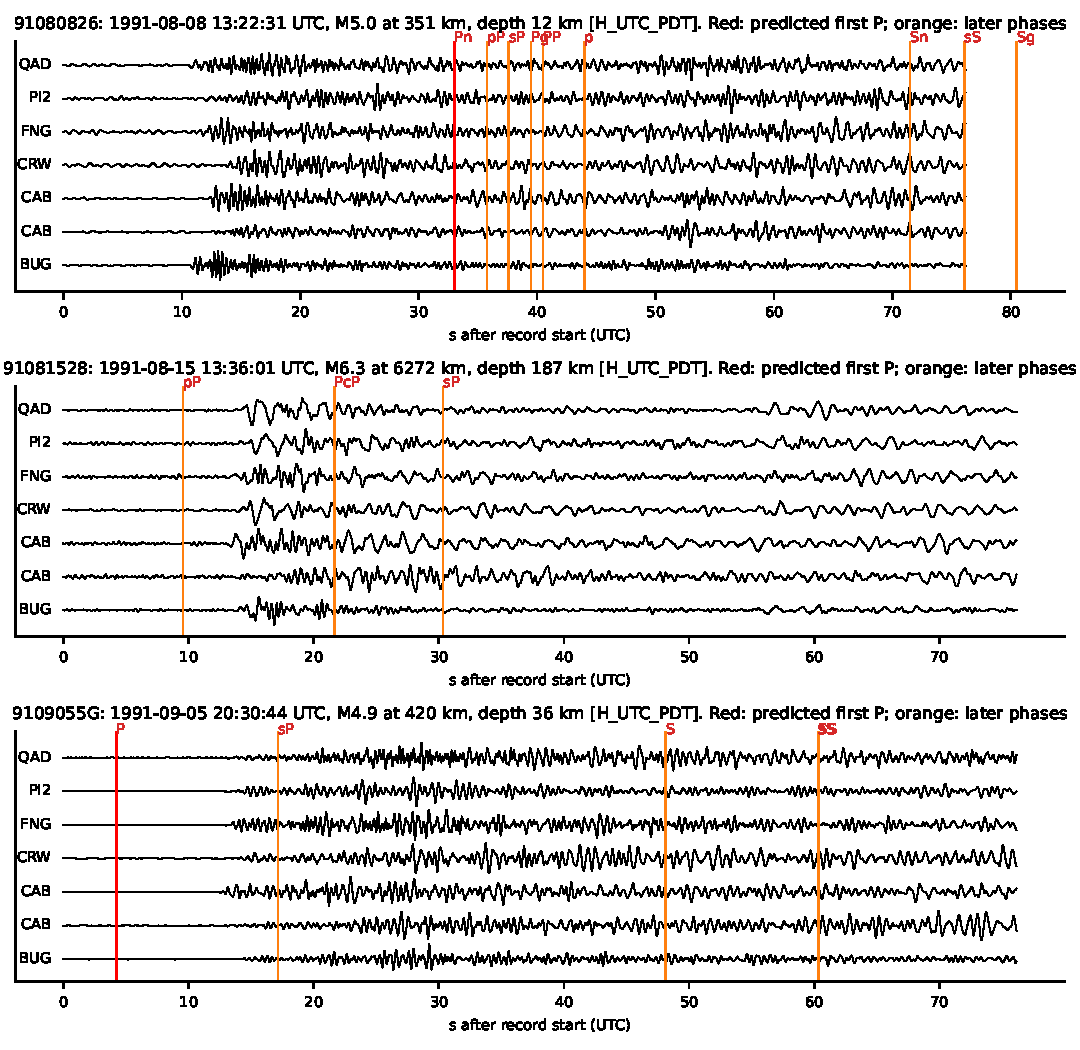
\includegraphics[width=\textwidth]{figS04_anchors_aug_sep}
\caption{Clock anchors, August--September 1991: records 91080826, 91081528 (offset measured from pP; the record starts after the predicted P) and 9109055G.}
\label{fig:anchors2}
\end{figure}

\section{Coverage of every channel and product}\label{sec:coverage}

Figure~3 of the main article shows coverage by data type. Figures~\ref{fig:wfch}--\ref{fig:bobother} break it down by channel and by source series, on UTC days. A marked day means at least one record (waveforms) or at least one usable value (BOB); it does not mean continuous operation.

\begin{figure}[htbp]
\centering
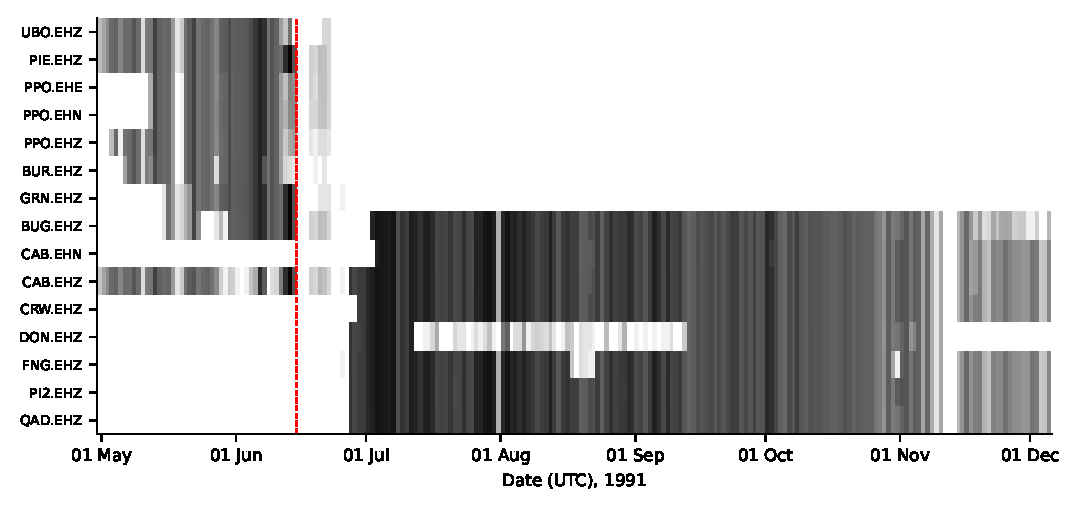
\includegraphics[width=\textwidth]{figS05_waveform_channels}
\caption{Triggered waveform traces per channel and UTC day (gray scale, logarithmic). Dashed line: 15 June.}
\label{fig:wfch}
\end{figure}

\begin{figure}[htbp]
\centering
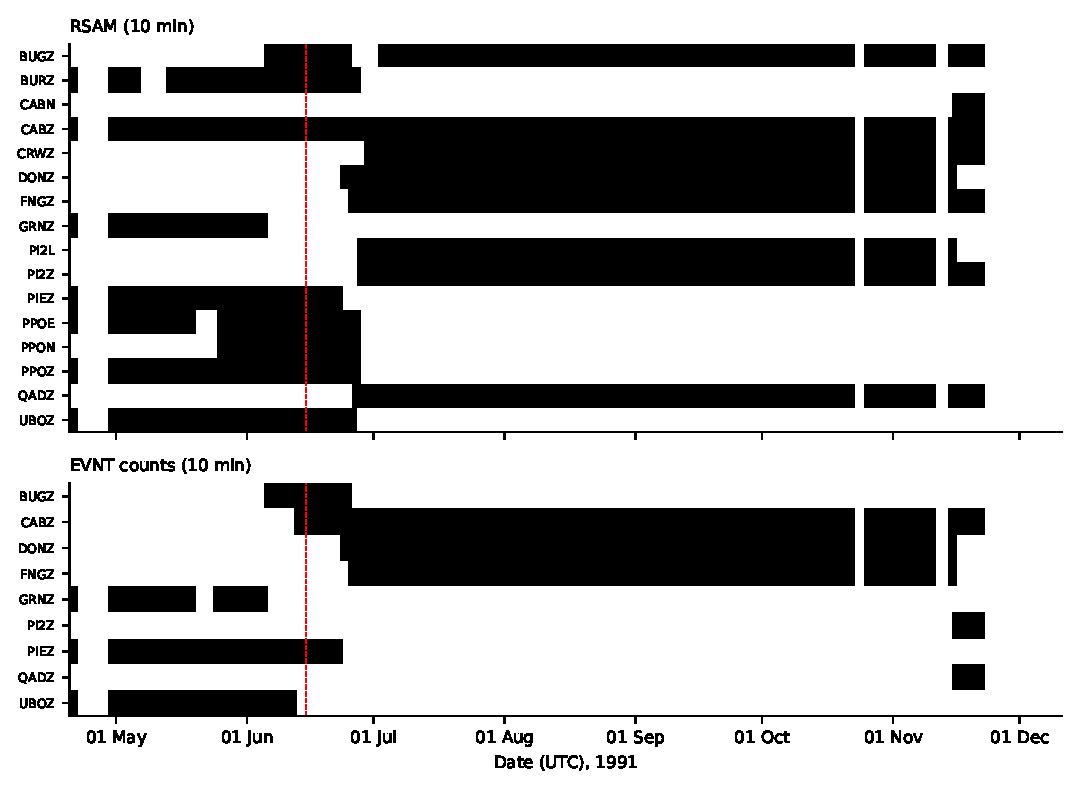
\includegraphics[width=\textwidth]{figS06_bob_rsam_evnt}
\caption{RSAM and EVNT by station channel: UTC days with at least one usable 10-minute value.}
\label{fig:bobrsam}
\end{figure}

\begin{figure}[htbp]
\centering
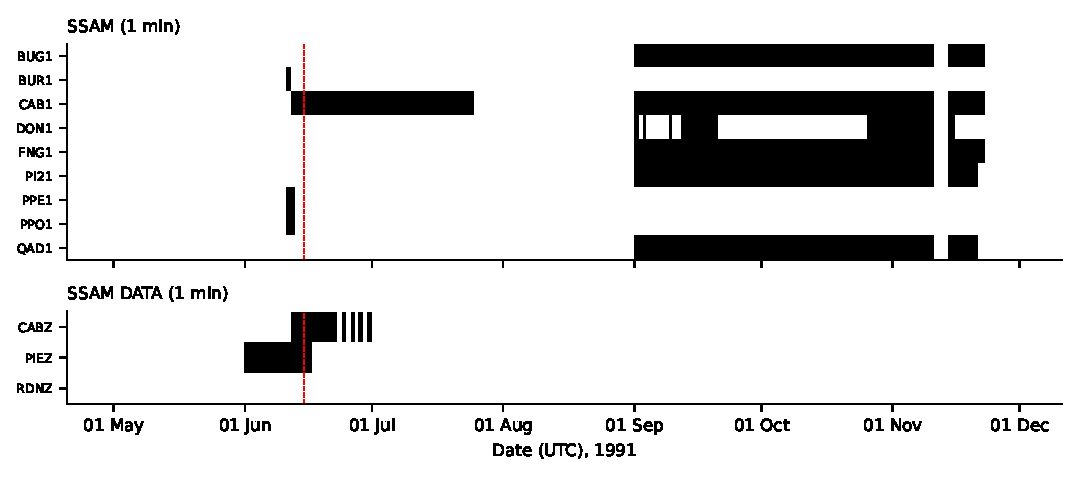
\includegraphics[width=\textwidth]{figS07_bob_ssam}
\caption{SSAM and SSAM DATA by source series: UTC days with at least one usable 1-minute value.}
\label{fig:bobssam}
\end{figure}

\begin{figure}[htbp]
\centering
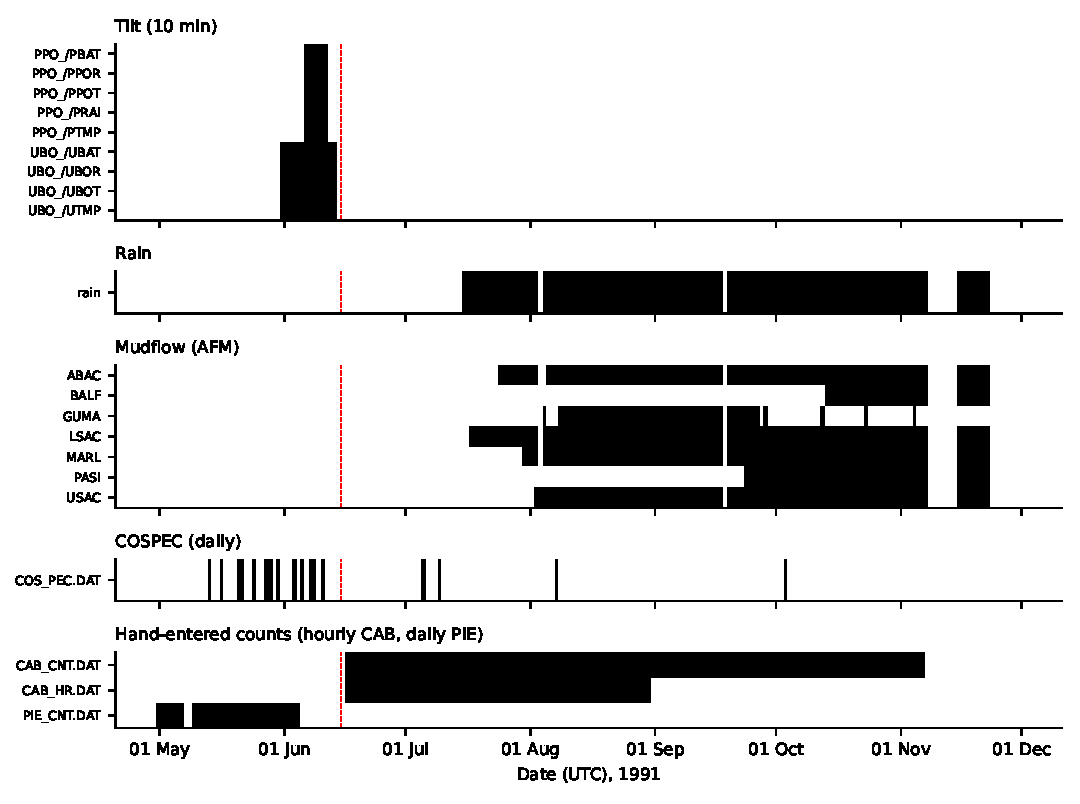
\includegraphics[width=\textwidth]{figS08_bob_other}
\caption{Tilt (PPO and UBO tilt, battery and temperature channels), rain, mudflow (acoustic flow monitors), COSPEC, and the hand-entered hourly CAB and daily PIE counts, by series. COSPEC dates are taken as Philippine days; rain and mudflow after 15 November are unverified (main article, Limitations).}
\label{fig:bobother}
\end{figure}

\section{Picks, locations and catalog}\label{sec:qc}

The two HYPO71 summaries share most events but not all solutions. For the 3,500 hypocenter groups with an origin in both, Figure~\ref{fig:hyposrc} shows how they differ; 757 are identical in time, epicenter and depth. Figures~\ref{fig:ps} and~\ref{fig:rea} are quality-control outputs of steps 23 and 53.

\begin{figure}[htbp]
\centering
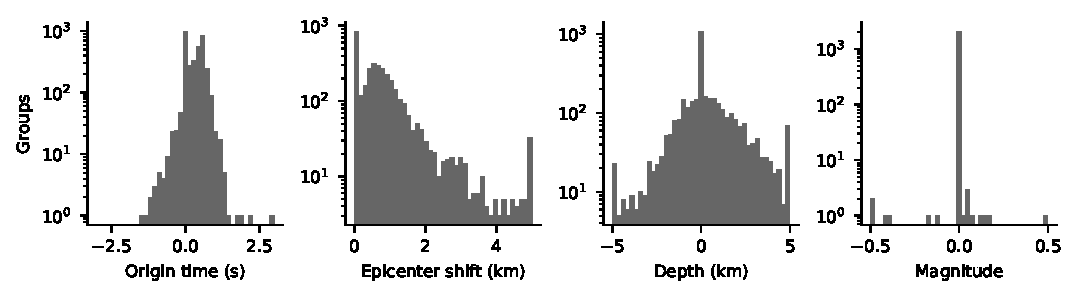
\includegraphics[width=\textwidth]{figS09_hypo_sources}
\caption{Differences between the two summaries for the same hypocenter group (\file{PINAALL.DAT} minus \file{Pinatubo\_all.sum}): origin time, epicenter shift, depth and magnitude. Values beyond the plotted range are placed in the end bins.}
\label{fig:hyposrc}
\end{figure}

\begin{figure}[htbp]
\centering
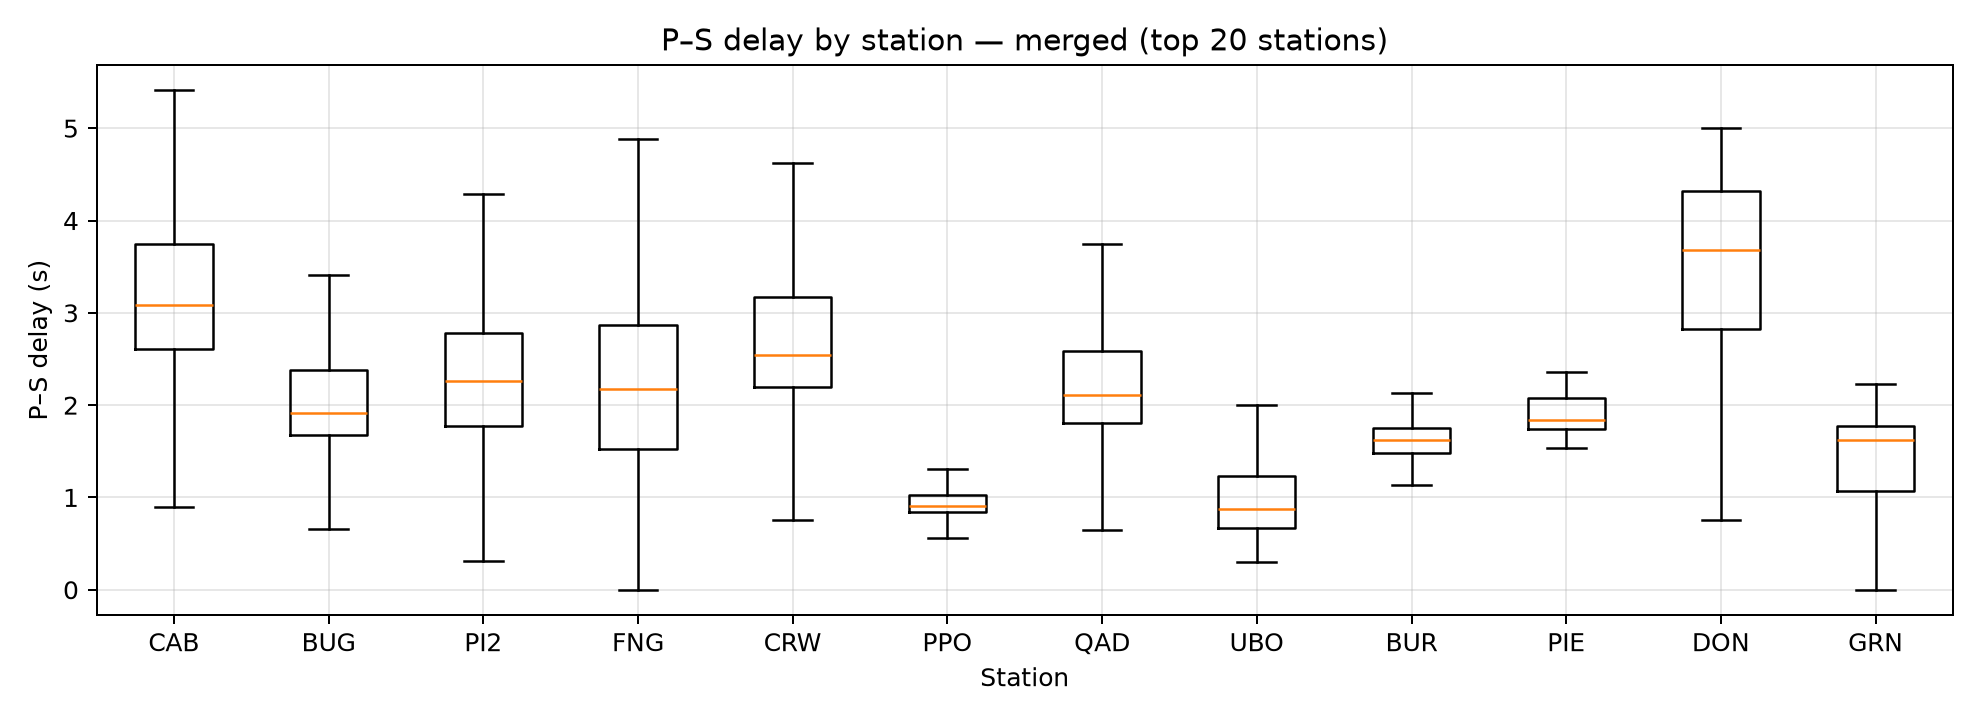
\includegraphics[width=0.85\textwidth]{figS10_ps_by_station}
\caption{S$-$P times by station for the merged picks (step 23).}
\label{fig:ps}
\end{figure}

\begin{figure}[htbp]
\centering
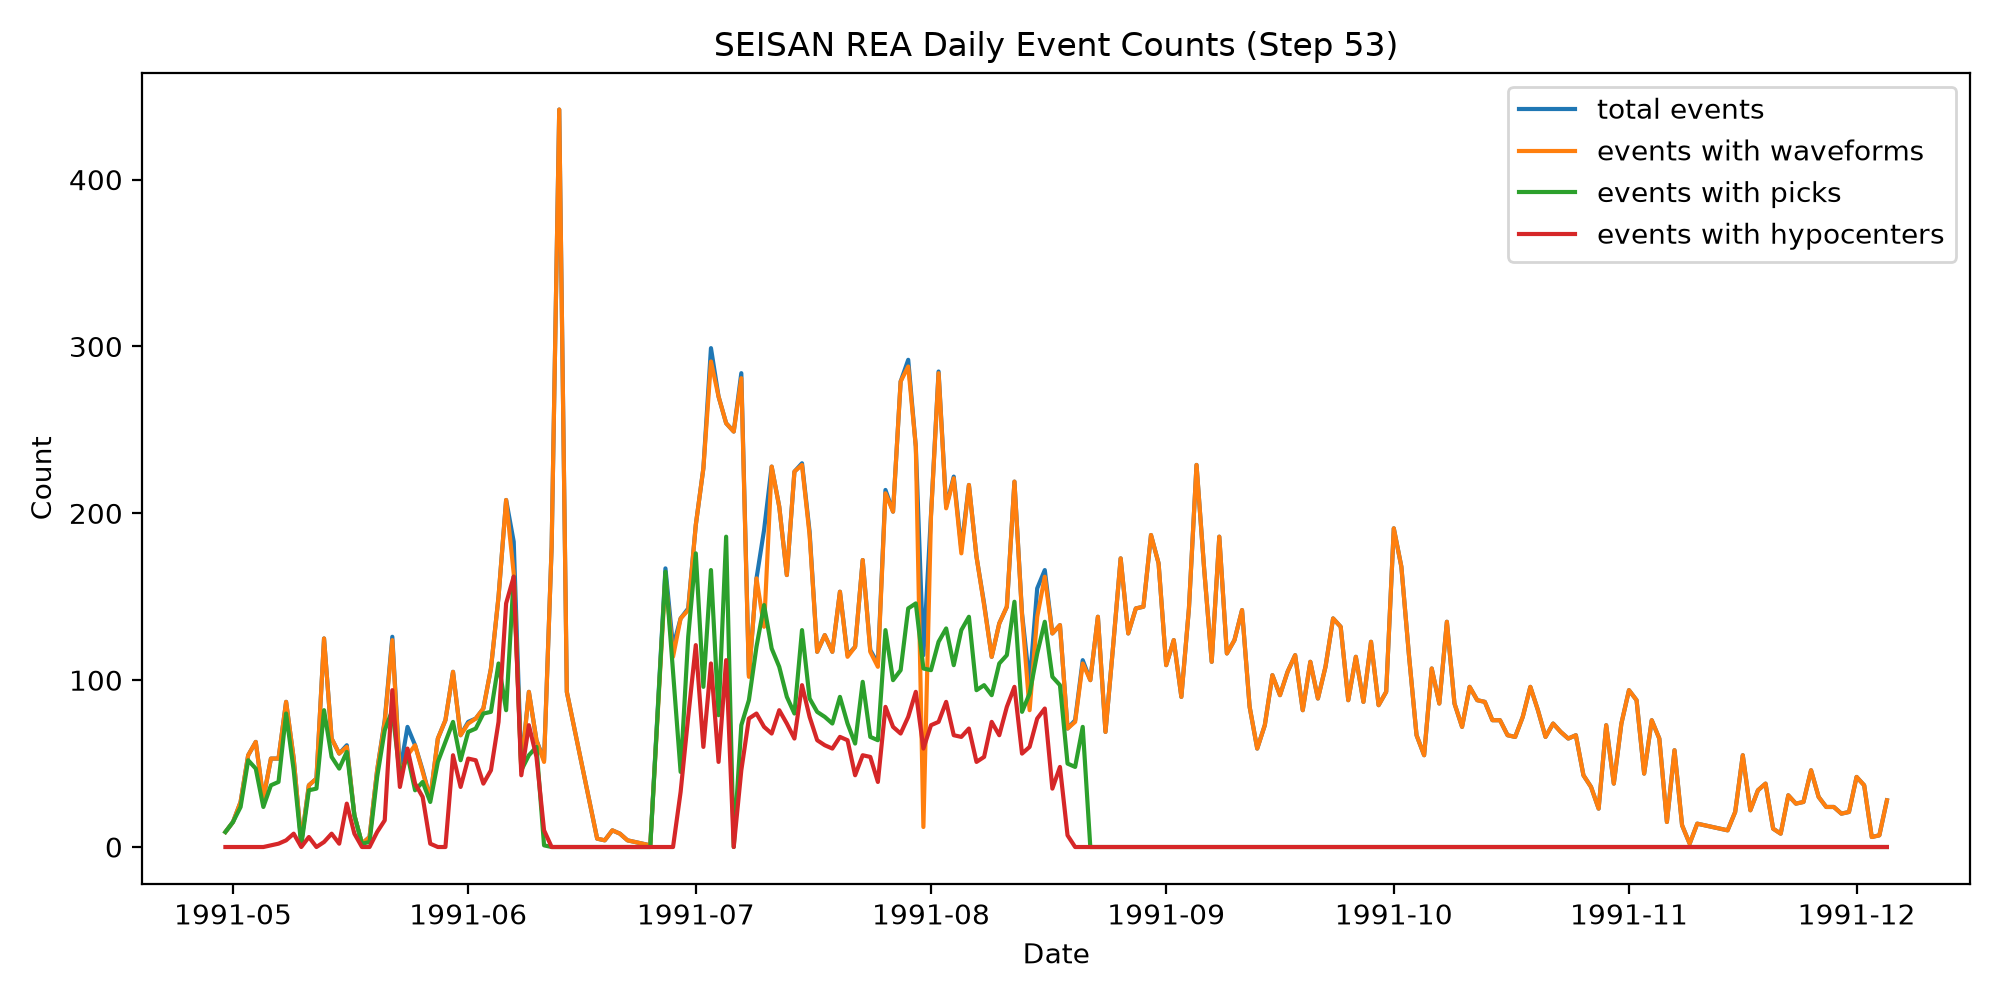
\includegraphics[width=0.85\textwidth]{figS11_rea_daily_counts}
\caption{Events per day in the written SEISAN REA database (step 53), checked against the catalog it was written from.}
\label{fig:rea}
\end{figure}

\section{Analysis workflow examples}\label{sec:analysis}

Figures~\ref{fig:noise} and~\ref{fig:spec} are produced by the analysis notebooks (run \texttt{45e939498e85}). The spectrogram example is from a draft selection of examples that has not yet been reviewed for publication.


\begin{figure}[htbp]
\centering
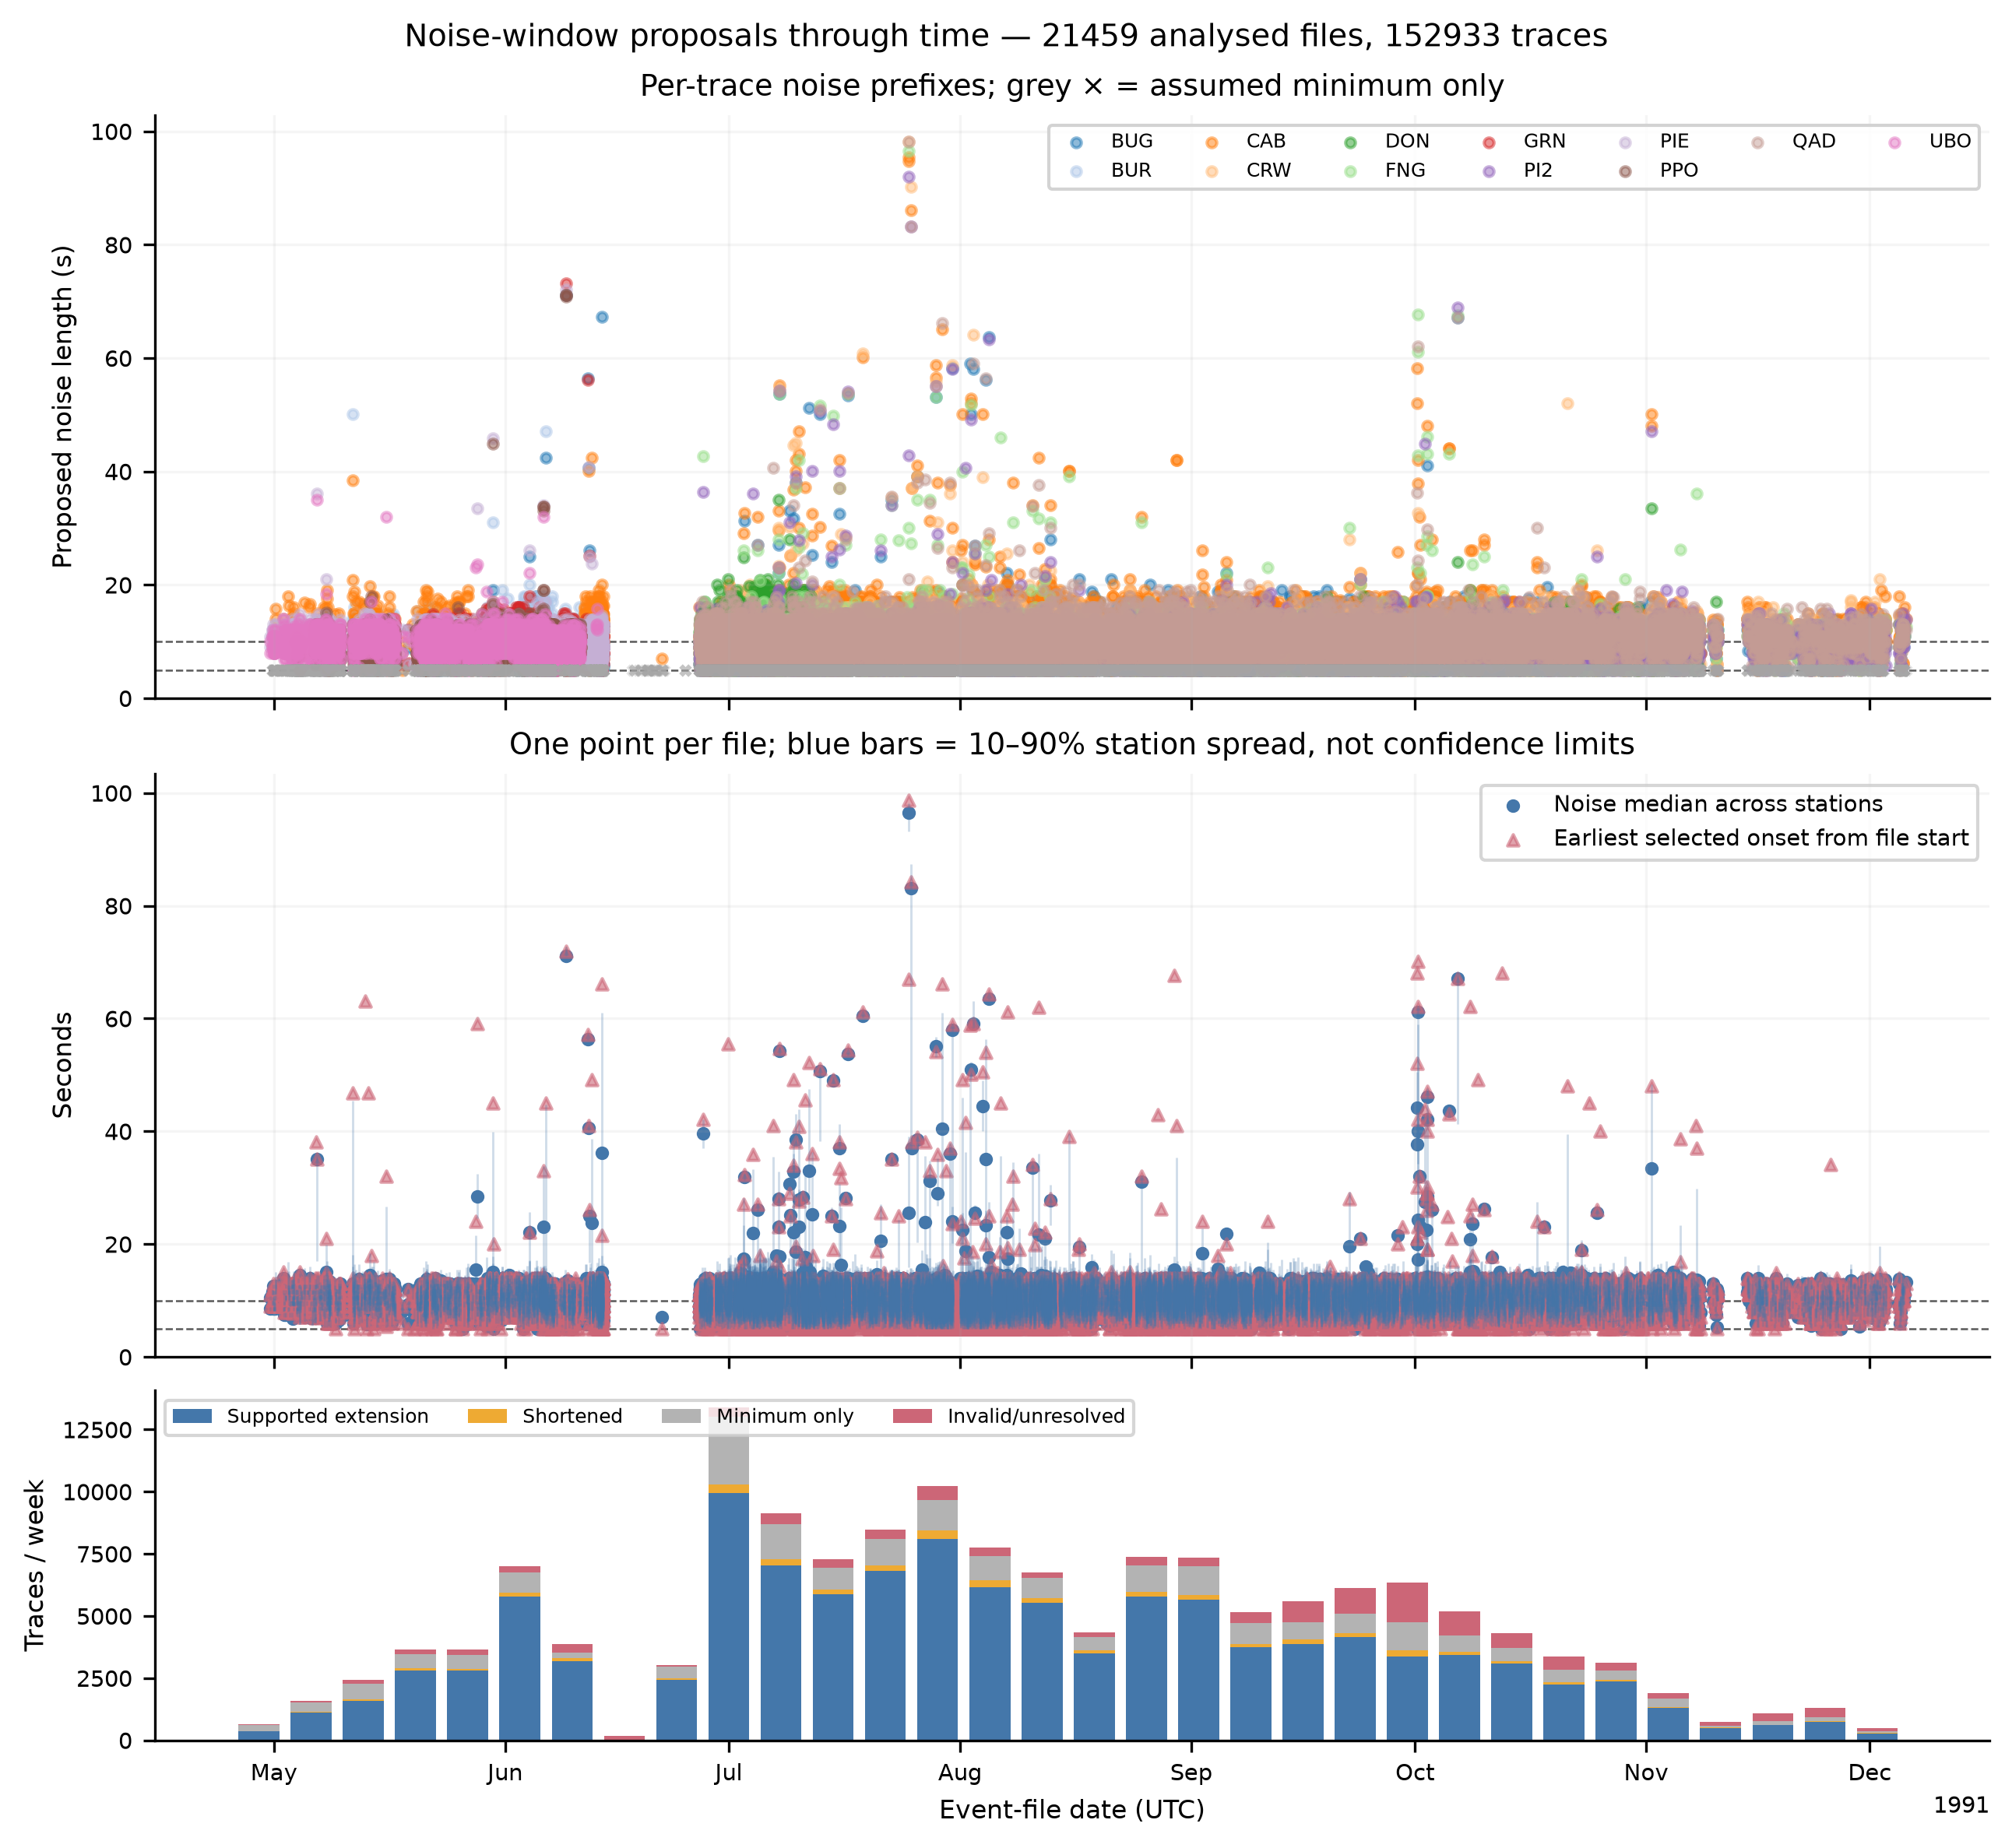
\includegraphics[width=\textwidth]{figS12_noise_windows}
\caption{Initial-noise window lengths through time (analysis notebook 20). These are proposed noise lengths before a detected onset, not the acquisition pretrigger setting; dashed 5- and 10-s lines are references.}
\label{fig:noise}
\end{figure}

\begin{figure}[htbp]
\centering
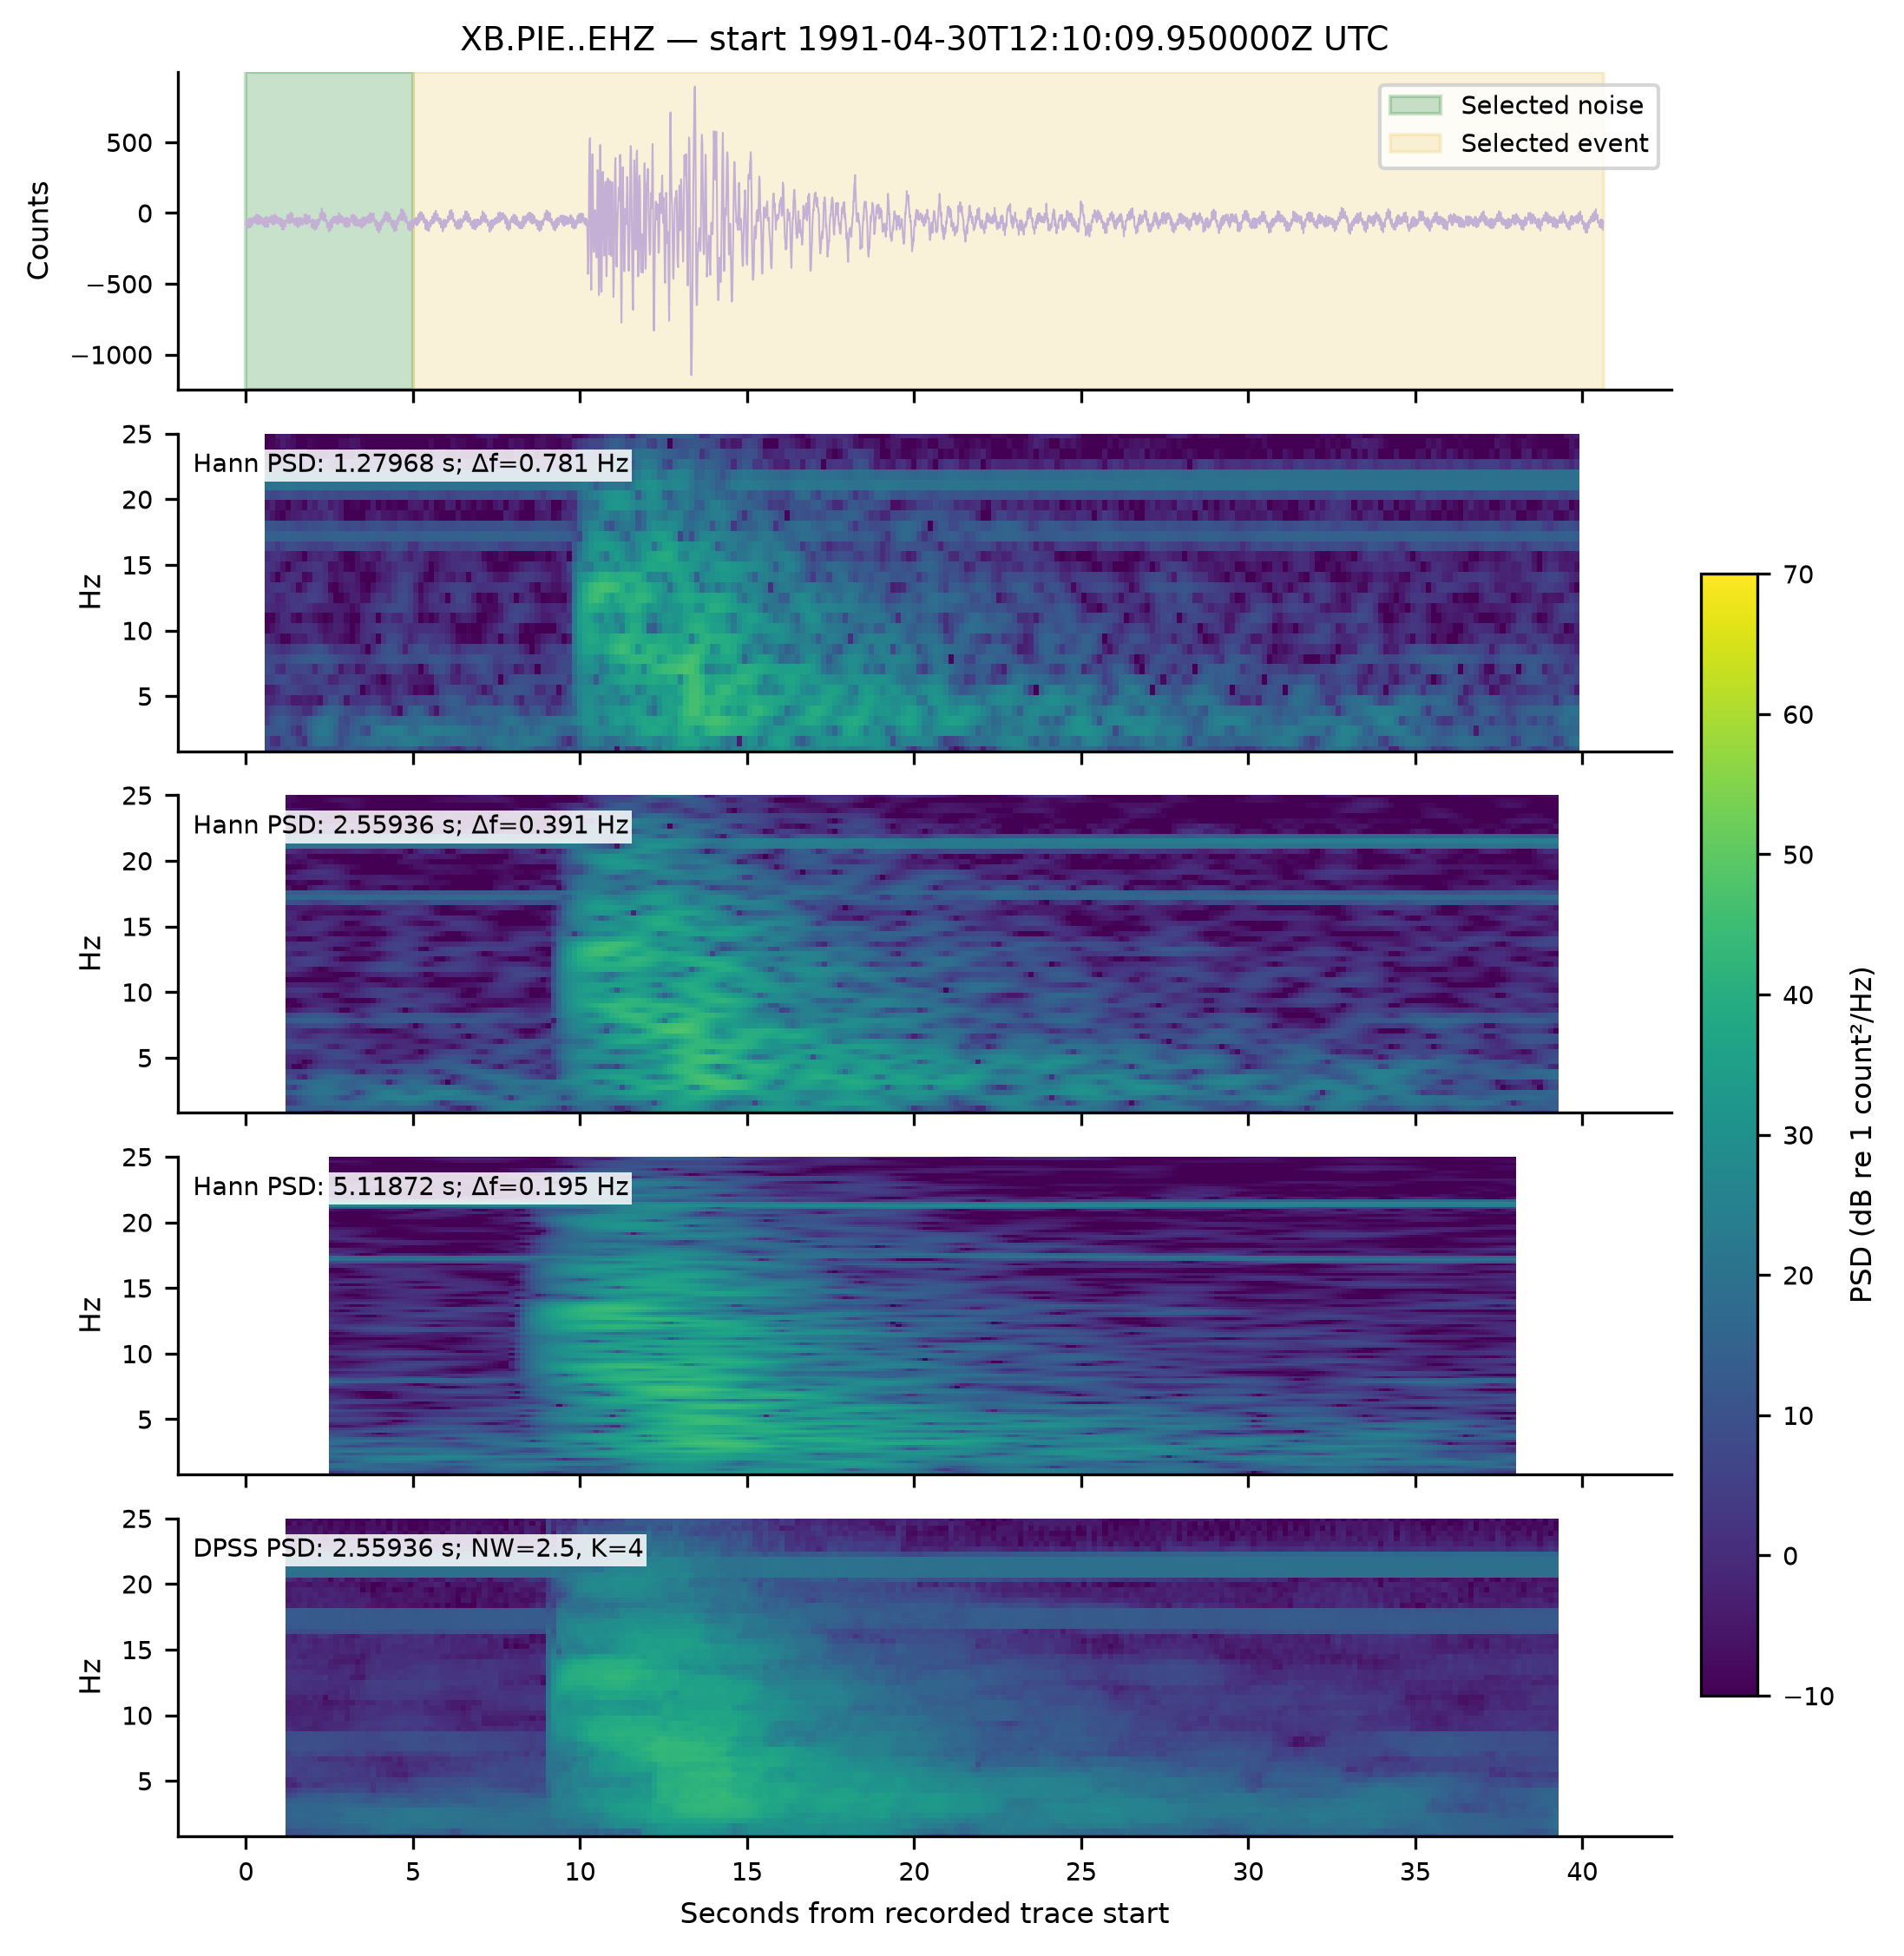
\includegraphics[width=\textwidth]{figS13_example_spectrograms}
\caption{Example spectrograms of one PIEZ record at several window lengths (analysis notebook 60, draft selection), in dB re 1~count$^2$/Hz with fixed color limits; shading marks the selected noise and event windows.}
\label{fig:spec}
\end{figure}

\bibliographystyle{../SSAbib}
\bibliography{../pinatubo}

\end{document}
